\documentclass[11pt]{article}
\topmargin=0.0in %length of margin at the top of the page (1 inch added by default)
\oddsidemargin=0.0in %length of margin on sides for odd pages
\evensidemargin=0in %length of margin on sides for even pages
\textwidth=6.5in %How wide you want your text to be
\marginparwidth=0.5in
\headheight=0pt %1in margins at top and bottom (1 inch is added to this value by default)
\headsep=0pt %Increase to increase white space in between headers and the top of the page
\textheight=9in %How tall the text body is allowed to be on each page

%
\usepackage{makeidx}  % allows for indexgeneration
\usepackage{amsmath}
\usepackage{listings}
\usepackage{algorithm}
\usepackage{algorithmic}
\usepackage{amsthm}
\usepackage{graphicx}
\usepackage{url}

\newtheorem{defn}{Definition}
\newtheorem{lemma}{Lemma}

\lstdefinelanguage{scala}{morekeywords={class,object,trait,extends,with,new,if,while,for,def,val,var,this},
otherkeywords={->,=>},
sensitive=true,
morecomment=[l]{//},
morecomment=[s]{/*}{*/},
morestring=[b]"}
% Default settings for code listings
\lstset{frame=tb,language=scala,aboveskip=3mm,belowskip=3mm,showstringspaces=false,columns=flexible,basicstyle={\small\ttfamily}}
%

\begin{document}

\title{Fast, Parallel INDEL Discovery \\ With Bubble Flank Motifs}
\author{Frank~Austin~Nothaft \\
Department of Electrical Engineering and Computer Sciences\\
University of California, Berkeley \\ 
Berkeley, CA 94720, USA \\
fnothaft@berkeley.edu}

\maketitle

\begin{abstract}

One of the primary challenges in variant calling is the discovery of short
insertion/deletion variants. These variants are difficult to call because the
reads that contain these variants are frequently misaligned around the variant.
To improve variant calling accuracy for short insertions and deletions, several
tools have switched to use local assembly based approaches. Local assemblers
detect areas of the reference genome that appear to be poorly aligned, and
call variants by performing de novo assembly on these regions. While local
assembly greatly improves variant calling accuracy, it has a substantial runtime
cost. In this paper, we introduce an algorithm that uses insight gained from
the structure of a colored de Bruijn graph to realign individual reads. We
prove that this algorithm has lower runtime complexity than traditional local
assembly approaches, while also providing canonical alignments for an individual
sequence variant. We demonstrate this algorithm in the open source, parallel
variant caller Avocado, which is available from
\url{https://github.com/bigdatagenomics/avocado}.

\end{abstract}

\section{Introduction}
\label{sec:introduction}

While many modern short-read based variant callers can achieve greater than
99\% accuracy when calling single nucleotide variants~(SNVs), accuracy decreases
when calling insertion/deletion~(INDEL) variants. For INDELs that are shorter
than the read length, some degradation in accuracy is caused by incorrect
mapping of reads containing INDELs. However, this is not the primary culprit.
As we show in~\S\ref{fixme} with a synthetic experiment, the majority of reads
that contain short INDELs map correctly. While these reads map correctly, they
are frequently locally misaligned. In short, these reads have been placed in
the correct area of the reference genome, but their local alignment makes them
appear to represent a different sequence variant then they truly contain.

There are two general approaches that can be used to eliminate the effect of
incorrect local alignment on variant calling accuracy: we can either use a local
sequence alignment algorithm that is less likely to misrepresent INDEL variants
when aligning individual reads, or we can try to improve the alignments of all
reads that have mapped around a genomic locus by pooling and jointly realigning
these reads. Most tools have focused on the second approach, which further
bifurcates into realignment-only and reassembly-with-realignment algorithms.
Research has focused on realignment-based approaches because realignment-based
approaches obliviate the major problem with traditional local sequence alignment
algorithms~\cite{smith81, ukkonen85, laundau86}, which by their probabilistic or
dynamic nature cannot be guaranteed to emit consistent alignments for all reads
that contain an INDEL variant~\cite{liFIXME}. Realignment algorithms eliminate
this problem by identifying all possible INDELs in the reads at the site,
scoring these variants at the site, and realigning the reads to contain a
consistent representation of the top scoring variant(s).

Although realignment and reassembly algorithms have high accuracy, they also
have high computational cost. The traditional formulation of a realignment
algorithm has $\mathcal{O}(n^4)$ runtime complexity, while most local sequence
alignment algorithms have runtime complexity of $\mathcal{O}(n^2)$ or lower.
Additionally, realignment approaches require all of the reads covering a
genomic locus to be materialized which necessitates a shuffle of the input
dataset and can have significant memory requirements. While the end-to-end
runtime can be decreased by only reassembling a portion of the genome, the
performance improvements available through these approaches are bound similarly
to Amdahl's law: local assembly is sufficiently expensive that an approach that
prefilters 90\% of the genome only achieves a $3\times$ improvement in
end-to-end runtime~\cite{bloniarz14}.

As an alternative to traditional realignment and reassembly approaches, we
introduce a local sequence alignment algorithm that is inspired by colored de
Bruijn graphs~\cite{iqbal12}. This algorithm has several desirable properties:
it has linear runtime complexity and it produces provably canonical pairwise
alignments. When used for locally realigning previously mapped reads, we can
determine if an individual read is already canonically aligned prior to
realigning, which allows us to aggressively limit the number of reads realigned.
Our algorithm uses motifs that we have identified in the structure of the
sequence flanking a bubble in a colored de Bruijn graph. Our algorithm has an
efficient implementation and we can prove strong guarantees about the local
alignments that our algorithm generates. We have implemented this algorithm in
\textsc{Avocado}, a parallel variant caller implemented using \textsc{Apache
Spark}~\cite{zaharia12, zaharia10} and the \textsc{ADAM} library for parallel
genomic analysis~\cite{massie13, nothaft15}. Our approach achieves a $10\times$
speedup over conventional INDEL realignment tools when run on a single node
while maintaining variant calling accuracy, and can be parallelized across a
cluster of computers. Our implementation is released as open source code under
an Apache 2 license and is available from
\url{https://github.com/bigdatagenomics/avocado}.

\section{Background}
\label{sec:background}

The accuracy of insertion and deletion~(INDEL) variant discovery has been improved by the development
of variant callers that couple local reassembly with haplotype-based statistical models to recover INDELs
that were locally misaligned~\cite{albers11}. Now, several prominent variant callers such as the Genome
Analysis Toolkit's~(GATK) \textsc{HaplotypeCaller}~\cite{depristo11}, \textsc{Scalpel}~\cite{narzisi14}, and
\textsc{Platypus}~\cite{rimmer14}. Although haplotype-based methods have enabled more accurate INDEL
and single nucleotide polymorphism~(SNP) calls~\cite{bao14}, this accuracy comes at the cost of
end-to-end runtime~\cite{talwalkar14}. Several recent projects have been focused on improving
reassembly cost either by limiting the percentage of the genome that is reassembled~\cite{bloniarz14} or
by improving the performance of algorithms of the core algorithms used in local
reassembly~\cite{rimmer14}.

The performance issues seen in haplotype reassembly approaches derives from the high asymptotic
complexity of reassembly algorithms. Although specific implementations may vary slightly, a typical
local reassembler performs the following steps:

\begin{enumerate}
\item A de Bruijn graph is constructed from the reads aligned to a region of the reference genome,
\item All valid paths~(\emph{haplotypes}) between the start and end of the graph are enumerated,
\item Each read is realigned to each haplotype, typically using a pair Hidden Markov Model~(HMM,
see~\cite{durbin98}),
\item A statistical model uses the read$\leftrightarrow$haplotype alignments to choose the haplotype pair
that most likely represents the variants hypothesized to exist in the region, 
\item The alignments of the reads to the chosen haplotype pair are used to generate statistics that are
then used for genotyping.
\end{enumerate}

In this paper, we focus on steps one through three of the local reassembly problem, as there is wide
variation in the algorithms used in stages four and five~(see~\S\ref{sec:background}). Stage one (graph
creation) has approximately $\mathcal{O}(r l_r)$ time complexity, and stage two (graph elaboration) has
$\mathcal{O}(h \max(l_h))$ time complexity.
The asymptotic time cost bound of local reassembly comes from stage three, where cost is $\mathcal{O}(h r l_r
\max(l_h))$, where $h$ is the number of haplotypes tested in this region\footnote{The number of
haplotypes tested may be lower than the number of haplotypes reassembled. Several tools
(see~\cite{depristo11,garrison12}) allow users to limit the number of haplotypes evaluated to improve
performance.}, $r$ is the number of reads aligned to this region, $l_r$ is the read length\footnote{For
simplicity, we assume constant read length. This is a reasonable assumption as many of the variant
callers discussed target Illumina reads that have constant length.}, and $\min(l_h)$ is the length of the
shortest haplotype that we are evaluating. This complexity comes from realigning $r$ reads to $h$
haplotypes, where realignment has complexity $\mathcal{O}(l_r l_h)$. We ignore the storage complexity of
reassembly here, but provide an extended
discussion of {de Bruijn} graph complexity in~\S\ref{sec:background}.

In this paper, we introduce the indexed de Bruijn graph and demonstrate how it can be used to
reduce the asymptotic complexity of reassembly. An indexed de Bruijn graph is identical to a
traditional de Bruijn graph, with one modification: when we create the graph, we annotate each
$k$-mer with the index position of that $k$-mer in the sequence it was observed in. This simple addition
enables the use of the indexed de Bruijn graph for $\Omega(n)$ local sequence alignment with
canonical edit representations for most edits. This structure can be used for both sequence alignment and
assembly, and achieves a more efficient approach for variant discovery via local reassembly.

Current variant calling pipelines depend heavily on realignment based approaches for accurate
genotyping~\cite{li14}. Although there are several approaches that do not make explicit use of reassembly,
all realignment based variant callers use an algorithmic structure similar to the one described
in~\S\ref{sec:introduction}. In non-assembly approaches like \textsc{FreeBayes}~\cite{garrison12}, stages
one and two are replaced with a single step where the variants observed in the reads aligned to a given
haplotyping region are filtered for quality and integrated directly into the reference haplotype in that region.
In both approaches, local alignment errors~(errors in alignment \emph{within} this region) are corrected
by using a statistical model to identify the most likely location that the read could have come from, given
the other reads seen in this area.

Although the model used for choosing the best haplotype pair to finalize realignments to varies between
methods~(e.g., the GATK's \textsc{IndelRealigner} uses a simple log-odds model~\cite{depristo11}, while
methods like \textsc{FreeBayes}~\cite{garrison12} and \textsc{Platypus}~\cite{rimmer14} make use of richer
Bayesian models), these methods require an all-pairs alignment of reads to candidate
haplotypes. This leads to the runtime complexity bound of $\mathcal{O}(h r l_r \min(l_h))$ given
in~\S\ref{sec:introduction}, as we must realign $r$ reads to $h$ haplotypes, where the cost of realigning
one read to one haplotype is $\mathcal{O}(l_r \max(l_h))$, where $l_r$ is the read length~(assumed to be
constant for Illumina sequencing data) and $\max(l_h)$ is the length of the longest haplotype. Typically,
the data structures used for realignment~($\mathcal{O}(l_r \max(l_h))$ storage cost) can be reused.
These methods typically retain \emph{only} the best local realignment per read per haplotype, thus
bounding storage cost at $\mathcal{O}(h r)$.

For non-reassembly based approaches, the cost of generating candidate haplotypes is $\mathcal{O}(r)$,
as each read must be scanned for variants, using the pre-existing alignment. These variants are typically
extracted from the CIGAR string, but may need to be normalized~\cite{li14}. de Bruijn graph based 
reassembly methods have similar $\mathcal{O}(r)$ time complexity for building the de Bruijn
graph as each read must be sequentially broken into $k$-mers, but these methods have a different
storage cost. Specifically, storage cost for a de Bruijn graph is similar to $\mathcal{O}(k
(l_{\text{ref}} + l_{\text{variants}} + l_{\text{errors}}))$, where $l_{\text{ref}}$ is the length of the reference
haplotype in this region, $l_{\text{variants}}$ is the length of true variant sequence in this region, 
$l_{\text{errors}}$ is the length of erroneous sequence in this region, and $k$ is the $k$-mer size. In
practice, we can approximate both errors and variants as being random, which gives $\mathcal{O}(k
l_{\text{ref}})$ storage complexity. From this graph, we must enumerate the haplotypes present in the
graph. Starting from the first $k$-mer in the reference sequence for this region, we perform a depth-first
search to identify all paths to the last $k$-mer in the reference sequence. Assuming that the graph is
acyclic~(a common restriction for local assembly, see~\S\ref{sec:limits-repeated-sequences}), we can
bound the best case cost of this search at $\Omega(h \min l_h)$.

The number of haplotypes evaluated, $h$, is an important contributor to the algorithmic complexity of
reassembly pipelines, as it sets the storage and time complexity of the realignment scoring phase, the
time complexity of the haplotype enumeration phase, and is related to the storage complexity of the
de Bruijn graph. The best study of the complexity of assembly techniques was done by Kingsford
et al.~\cite{kingsford10}, but is focused on \emph{de novo} assembly and pays special attention to
resolving repeat structure. In the local realignment case, the number of haplotypes identified is determined
by the number of putative variants seen. We can na\"{i}vely model this cost with \eqref{eq:haplotypes},
where $f_v$ is the frequency with which variants occur, $\epsilon$ is the rate at which bases are
sequenced erroneously, and $c$ is the coverage (read depth) of the region.

\begin{align}
\label{eq:haplotypes}
h \sim f_v l_{\text{ref}} + \epsilon l_{\text{ref}} c
\end{align}

This model is na\"{i}ve, as the coverage depth and rate of variation varies across sequenced datasets,
especially for targeted sequencing runs~\cite{fang14}. Additionally, while the $\epsilon$ term models the
total number of sequence errors, this is not completely correlated with the number of \emph{unique}
sequencing errors, as sequencing errors are correlated with sequence context~\cite{depristo11}. Many
current tools allow users to limit the total number of evaluated haplotypes, or apply strategies to minimize
the number of haplotypes considered, such as filtering observed variants that are likely to be sequencing
errors~\cite{garrison12}, restricting realignment to INDELs~(\textsc{IndelRealigner},~\cite{depristo11}), or
by trimming paths from the assembly graph. Additionally, in an de Bruijn graph, errors in the
first $k$ or last $k$ bases of a read will manifest as spurs~(see~\S\ref{sec:spurs}) and will not contribute paths through the graph. We provide~\eqref{eq:haplotypes} solely as a motivating
approximation, and hope to study these characteristics in more detail in future work.

\section{Method}
\label{sec:method}

As opposed to traditional realignment based approaches, we canonicalize INDELs
in the reads by looking for ``bubble flank motifs.'' In a colored de Bruijn
graph, a bubble refers to a location where the graph diverges between two
samples. In \S\ref{sec:formulation}, we demonstrate how we can use the
reconvergence of the de Bruijn graph in the flanking sequence around a bubble
to define provably canonical alignments of the bubble between two sequences.
For a colored de Bruijn graph containing reads and the reference genome, this
allows us to canonically express INDEL variants in the reads against the
reference. In \S\ref{sec:implementation}, we then show how this approach
can be implemented efficiently without building a de Bruijn graph per read,
or even adding each read to a de Bruijn graph.

\subsection{Preliminaries}
\label{sec:formulation}

Our method relies on an \emph{indexed de Bruijn} graph, which is a slight
extension of the colored de Bruijn graph~\cite{iqbal12}. Specifically, each
$k$-mer in an indexed de Bruijn graph knows which sequence position~(index)
it came from in it's underlying read/sequence. To construct an indexed de
Bruijn graph, we start with the traditional formulation of a \emph{de Brujin}
graph for sequence assembly:

\begin{defn}[de Bruijn Graph]
\label{defn:dbg}
A de Bruijn graph describes the observed transitions between adjacent $k$-mers in a sequence. Each
$k$-mer $s$ represents a $k$-length string, with a $k - 1$ length prefix given by $\text{prefix}(s)$ and a
length 1 suffix given by $\text{suffix}(s)$. We place a directed edge ($\rightarrow$) from $k$-mer $s_1$ to
$k$-mer $s_2$ if $\text{prefix}(s_1)^{\{1, k - 2\}} + \text{suffix}(s_1) = \text{prefix}(s_2)$.
\end{defn}

Now, suppose we have $n$ sequences $\mathcal{S}_1, \dots, \mathcal{S}_n$. Let us assert that for each
$k$-mer $s \in \mathcal{S}_i$, then the output of function $\text{index}_i(s)$ is defined. This function
provides us with the integer position of $s$ in sequence $\mathcal{S}_i$. Further, given two $k$-mers
$s_1, s_2 \in \mathcal{S}_i$, we can define a distance function
$\text{distance}_i(s_1, s_2) = | \text{index}_i(s_1) - \text{index}_i(s_2) |$. To create an indexed
de Bruijn graph, we simply annotate each $k$-mer $s$ with the $\text{index}_i(s)$ value for all
$\mathcal{S}_i, i \in \{1, \dots, n\}$ where $s \in \mathcal{S}_i$. This index value is trivial to log when
creating the original de Bruijn graph from the provided sequences.

Let us require that all sequences $\mathcal{S}_1, \dots, \mathcal{S}_n$ are not repetitive, which implies
that the resulting de Bruijn graph is acyclic. If we select any two sequences $\mathcal{S}_i$ and
$\mathcal{S}_j$ from $\mathcal{S}_1, \dots, \mathcal{S}_n$ that share at least two $k$-mers $s_1$ and
$s_2$ with common ordering~($s_1 \rightarrow \dots \rightarrow s_2$ in both $\mathcal{S}_i$ and
$\mathcal{S}_j$), the indexed de Bruijn graph $G$ provides several guarantees:

\begin{enumerate}
\item If two sequences $\mathcal{S}_i$ and $\mathcal{S}_j$ share at least two $k$-mers $s_1$ and
$s_2$, we can provably find the maximum edit distance $d$ of the subsequences in $\mathcal{S}_i$ and
$\mathcal{S}_j$, and bound the cost of finding this edit distance at $\mathcal{O}(nd)$,\footnote{Here,
$n = \max(\text{distance}_{\mathcal{S}_i}(s_1, s_2), \text{distance}_{\mathcal{S}_j}(s_1, s_2))$.}
\item For many of the above subsequence pairs, we can bound the cost at $\mathcal{O}(n)$, \emph{and}
provide canonical representations for the necessary edits,
\item $\mathcal{O}(n^2)$ complexity is restricted to aligning the subsequences of $\mathcal{S}_i$ and
$\mathcal{S}_j$ that exist \emph{before} $s_1$ or \emph{after} $s_2$.
\end{enumerate}

Let us focus on cases 1 and 2, where we are looking at the subsequences of $\mathcal{S}_i$ and
$\mathcal{S}_j$ that are between $s_1$ and $s_2$. A trivial case arises when both $\mathcal{S}_i$ and
$\mathcal{S}_j$ contain an identical path between $s_1$ and $s_2$ (i.e.,
$s_1 \rightarrow s_n \rightarrow \dots \rightarrow s_{n + m} \rightarrow s_2$ and
$s_{n + k} \in \mathcal{S}_i \wedge s_{n + k} \in \mathcal{S}_j \forall k \in \{0, \dots , m\}$). Here, the
subsequences are clearly identical. This determination can be made trivially by walking from vertex $s_1$
to vertex $s_2$ with $\mathcal{O}(m)$ cost.

However, three distinct cases can arise whenever $\mathcal{S}_i$ and $\mathcal{S}_j$ diverge between
$s_1$ and $s_2$. For simplicity, let us assume that both paths are independent~(see
Definition~\ref{defn:path-independence}). These three cases correspond to there being either a canonical
substitution edit, a canonical INDEL edit, or a non-canonical (but known distance) edit between
$\mathcal{S}_i$ and $\mathcal{S}_j$.

\begin{defn}[Path Independence]
\label{defn:path-independence}
Given a non-repetitive de Bruijn graph $G$ constructed from $\mathcal{S}_i$ and $\mathcal{S}_j$, we say
that $G$ contains independent paths between $s_1$ and $s_2$ if we can construct two subsets
$\mathcal{S}'_i \subset \mathcal{S}_i, \mathcal{S}'_j \subset \mathcal{S}_j$ of $k$-mers where $s_{i + n}
\in \mathcal{S}'_i \forall n \in \{0, \dots, m_i\}, s_{i + n - 1} \rightarrow s_{i + n} \forall n \in \{1, \dots, m_i\}$,
$s_{j + n} \in \mathcal{S}'_j \forall n \in \{0, \dots, m_j\}, s_{j + n - 1} \rightarrow s_{j + n} \forall n \in \{1,
\dots, m_j\}$, and $s_1 \rightarrow s_i, s_j; s_{i + m_i}, s_{j + m_j} \rightarrow s_2$ and $\mathcal{S}'_i
\bigcap \mathcal{S}'_j = \emptyset$, where $m_i = \text{distance}_{\mathcal{S}_i}(s_1, s_2)$, and $m_j =
\text{distance}_{\mathcal{S}_j}(s_1, s_2)$. This implies that the sequences $\mathcal{S}_i$ and
$\mathcal{S}_j$ are different between $s_1, s_2$,
\end{defn}

We have a canonical substitution edit if $m_i = m_j = k$, where $k$ is the $k$-mer size. Here, we can
prove that the edit between $\mathcal{S}_i$ and $\mathcal{S}_j$ between $s_1, s_2$ is a single base
substitution $k$ letters after $\text{index}(s_1)$:

\begin{proof}[Proof regarding Canonical Substitution]
\label{proof:canonical-substitution}
Suppose we have two non-repetitive sequences, $\mathcal{S}_i'$ and $\mathcal{S}_j'$, each of length
$2k + 1$. Let us construct a de Bruijn graph $G$, with $k$-mer length $k$. If each sequence begins with
$k$-mer $s_1$ and ends with $k$-mer $s_2$, then that implies that the first and last $k$ letters of
$\mathcal{S}_i'$ and $\mathcal{S}_j'$ are identical. If both subsequences had the same character at
position $k$, this would imply that both sequences were identical and therefore the two paths between
$s_1, s_2$ would not be independent~(Definition~\ref{defn:path-independence}). If the two letters are
different \emph{and} the subsequences are non-repetitive, each character is responsible for $k$
previously unseen $k$-mers. This is the only possible explanation for the two independent $k$ length
paths between $s_1$ and $s_2$.
\end{proof}

To visualize the graph corresponding to a substitution, take the two example sequences \texttt{CCACTGT}
and \texttt{CCAATGT}. These two sequences differ by a \texttt{C} $\leftrightarrow$ \texttt{A} edit at
position three. With $k$-mer length $k = 3$, this corresponds to the graph in Figure~\ref{fig:sne}.

\begin{figure}[h]
\begin{center}
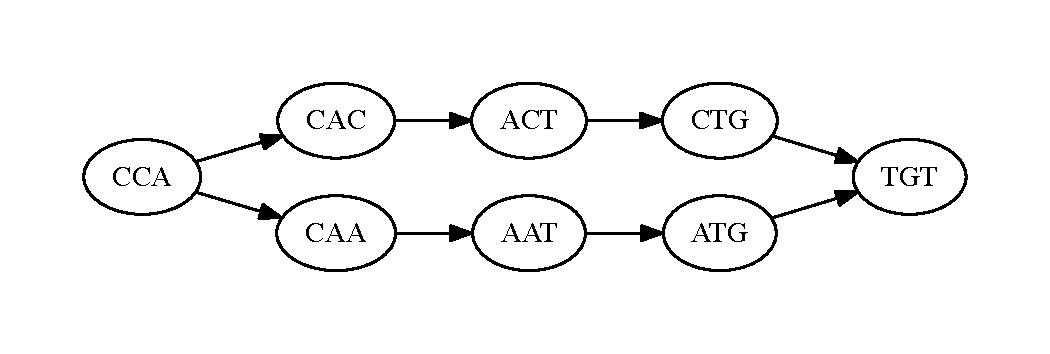
\includegraphics[width=0.5\linewidth, clip=true, trim=0 39 0 39]{graphs/sne.pdf}
\end{center}
\caption{Subgraph Corresponding To a Single Nucleotide Edit}
\label{fig:sne}
\end{figure}

If $m_i = k - 1, m_j \ge k$ or vice versa, we have a canonical INDEL edit (for convenience, we assume
that $\mathcal{S}_i'$ contains the $k - 1$ length path). Here, we can prove that there is a $m_j - m_i$
length insertion\footnote{This is equivalently a $m_j - m_i$ length deletion in $\mathcal{S}_i'$ relative to
$\mathcal{S}_j'$.} in $\mathcal{S}_j'$ relative to $\mathcal{S}_i'$, $k - 1$ letters \emph{after}
$\text{index}(s_1)$:

\begin{lemma}[Distance between $k$ length subsequences]
\label{lem:minimum-distance}
\emph{Indexed de Bruijn} graphs naturally provide a distance metric for $k$ length substrings. Let us construct an
indexed de Bruijn graph $G$ with $k$-mers of length $k$ from a non-repetitive sequence $\mathcal{S}$.
For any two $k$-mers $s_a, s_b \in \mathcal{S}, s_a \ne s_b$, the
$\text{distance}_\mathcal{S}(s_a, s_b)$ metric is equal to $l_p + 1$, where $l_p$ is the length of the
path (in $k$-mers) between $s_a$ and $s_b$. Thus, $k$-mers with overlap of $k - 1$ have an edge
directly between each other ($l_p = 0$) and a distance metric of 1. Conversely, two $k$-mers that are
adjacent but not overlapping in $\mathcal{S}$ have a distance metric of $k$, which implies $l_p = k - 1$.
\end{lemma}

\begin{proof}[Proof regarding Canonical INDELs]
\label{proof:canonical-indels}
We are given a graph $G$ which is constructed from two non-repetitive sequences $\mathcal{S}_i'$ and
$\mathcal{S}_j'$, where the only two $k$-mers in both $\mathcal{S}_i'$ and $\mathcal{S}_j'$ are $s_1$
and $s_2$ and both sequences provide independent paths between $s_1$ and $s_2$. By
Lemma~\ref{lem:minimum-distance}, if the path from $s_1 \rightarrow \dots \rightarrow s_2 \in
\mathcal{S}_i'$ has length $k - 1$, then $\mathcal{S}_i'$ is a string of length $2k$ that is formed by
concatenating $s_1, s_2$. Now, let us suppose that the path from $s_1 \rightarrow \dots \rightarrow s_2
\in \mathcal{S}_j'$ has length $k + l - 1$. The first $l$ $k$-mers after $s_1$ will introduce a $l$ length
subsequence $\mathcal{L} \subset \mathcal{S}_j', \mathcal{L} \not\subset \mathcal{S}_i'$, and then the
remaining $k - 1$ $k$-mers in the path provide a transition from $\mathcal{L}$ to $s_2$. Therefore,
$\mathcal{S}_j'$ has length of $2k + l$, and is constructed by concatenating $s_1, \mathcal{L}, s_2$.
This provides a canonical placement for the inserted sequence $\mathcal{L}$ in $\mathcal{S}_j'$ between
$s_1$ and $s_2$.
\end{proof}

To visualize the graph corresponding to a canonical INDEL, take the two example sequences
\texttt{CACTGT} and \texttt{CACCATGT}. Here, we have a \texttt{CA} insertion after position two. With
$k$-mer length $k = 3$, this corresponds to the graph in Figure~\ref{fig:indel}.

\begin{figure}[h]
\begin{center}
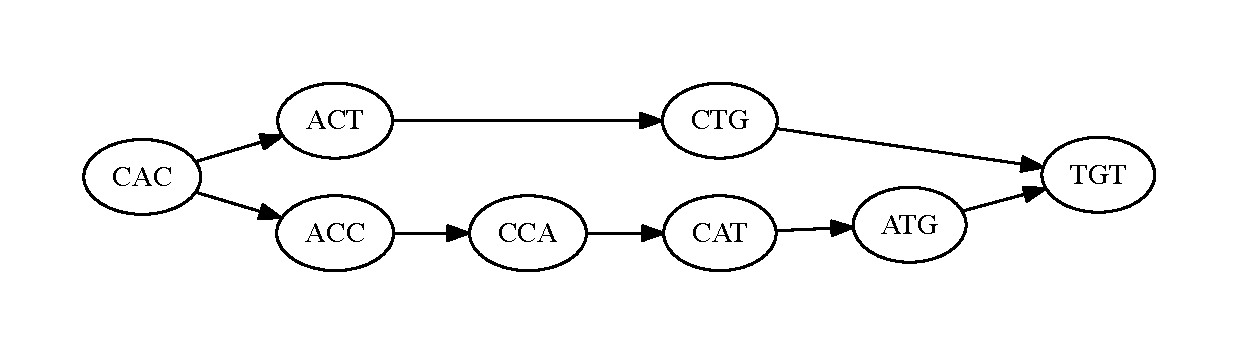
\includegraphics[width=0.5\linewidth, clip=true, trim=0 39 0 39]{graphs/indel.pdf}
\end{center}
\caption{Subgraph Corresponding To a Canonical INDEL Edit}
\label{fig:indel}
\end{figure}

Where we have a canonical allele, the cost of computing the edit is set by the need to walk the graph
linearly from $s_1$ to $s_2$, and is therefore $\mathcal{O}(n)$. However, in practice, we will see
differences that cannot be described as one of the earlier two canonical approaches. First, let us
generalize from the two above proofs: if we have two independent paths between $s_1, s_2$ in the
de Bruijn graph $G$ that was constructed from $\mathcal{S}_i, \mathcal{S}_j$, we can describe
$\mathcal{S}_i$ as a sequence created by concatenating $s_1, \mathcal{L}_i, s_2$.\footnote{This
property holds true for $\mathcal{S}_j$ as well.} The canonical edits merely result from special cases:

\begin{itemize}
\item In a canonical substitution edit, $l_{\mathcal{L}_i} = l_{\mathcal{L}_j} = 1$.
\item In a canonical INDEL edit, $l_{\mathcal{L}_i} = 0, l_{\mathcal{L}_j} \ge 1$.
\end{itemize}

Conceptually, a non-canonical edit occurs when two edits occur within $k$ positions of each other. In
this case, we can trivially fall back on a $O(nm)$ local alignment algorithm~(e.g., a pairwise HMM or
Smith-Waterman, see~\cite{durbin98,smith81}), \emph{but} we only need to locally realign
$\mathcal{L}_i$ against $\mathcal{L}_j$, which reduces the size of the realignment problem. However, we
can further limit this bound by limiting the maximum number of INDEL edits to $d = | l_{\mathcal{L}_i} -
l_{\mathcal{L}_j} |$. This allows us to use an alignment algorithm that limits the number of INDEL
edits~(e.g., Ukkonen's algorithm~\cite{ukkonen85}). By this, we can achieve $O(n(d + 1))$ cost.

\subsection{Implementation}
\label{sec:implementation}

\section{Results}
\label{sec:results}

\subsection{Accuracy}
\label{sec:accuracy}

To benchmark \textsc{Avocado}'s accuracy, we used the high coverage, PCR-free
whole genome sequencing~(WGS) run of NA12878 from the 1,000 Genomes
project~\cite{1kg}. We chose this dataset because NA12878 has extensive
orthogonal verification data that is available through the National Institute
for Standards and Time's~(NIST's) Genome-in-a-Bottle~(GIAB)
project~\cite{zook15}, and the WGS preparation of NA12878 for the 1,000 Genomes
project\footnote{The high coverage NA12878 data is available from
\url{ftp://ftp-trace.ncbi.nlm.nih.gov/1000genomes/ftp/phase3/data/NA12878/high_coverage_alignment/NA12878.mapped.ILLUMINA.bwa.CEU.high_coverage_pcr_free.20130906.bam}.}
is more representative of a typical sequencing dataset than the GIAB $300\times$
coverage WGS data for NA12878. We verified our calls using the Global Alliance
for Genomics and Health's~(GA4GH's) benchmarking suite\footnote{Available from
\url{https://github.com/ga4gh/benchmarking-tools}. Also, see Paten et
al~\cite{paten15}.} Since the NA12878 alignment available from 1,000 Genomes
represents the final, preprocessed analysis-ready reads, we realigned the reads
using \textsc{BWA}, before running the data through \textsc{Avocado},
\textsc{Samtools}/\textsc{Bcftools} \textsc{Mpileup}~\cite{danecek11, li11,
li09}, and the \textsc{GATK}'s \textsc{HaplotypeCaller}~\cite{depristo11}.
The relative accuracy of all three tools is shown in Table~\ref{tab:accuracy}.

\begin{table}[h]
\centering
\caption{Accuracy on NA12878}
\label{tab:accuracy}
\begin{tabular}{ l | c c c }
\hline
 & \bf \textsc{Mpileup} & \bf \textsc{GATK} & \bf \textsc{Avocado} \\
\hline
\hline
SNP Recall & & & 97\% \\
SNP Precision & & & 98\% \\
\hline
INDEL Recall & & & 55\% \\
INDEL Precision & & & 75\% \\
\hline
Runtime & & & 19h55m \\
\end{tabular}
\end{table}

\subsection{Performance}
\label{sec:performance}

Figure~\ref{fig:speedup}A demonstrates \textsc{Avocado}'s strong scaling. In
this experiment, we ran \textsc{Avocado}'s INDEL realigner and genotyper on a
constant dataset (the high coverage NA12878 dataset from 1,000
Genomes~\cite{1kg}), while varying the size of the cluster that \textsc{Avocado}
was run on. This experiment was run on our in-house cluster, which contains
64 machines connected by a full-bisection bandwidth 10 gigabit ethernet
network. Each machine in this cluster runs a 16-core Intel Xeon E5-2670 at
2.6GHz, with 256GB of memory. Each node has four 1TB hard disk
drives, and data was stored in the \textsc{Apache Hadoop Distributed File
System}~(HDFS,~\cite{shvachko10}). The cluster resources are managed by \textsc{Apache
YARN}~\cite{vavilapalli13}. We ran \textsc{Apache Hadoop} 2.6.2, and \textsc{Apache
Spark} 1.6.2. Due to cluster maintainance, several nodes were out of commission,
limiting us to 896 cores for our experiments.

\begin{figure}[h]
\begin{center}
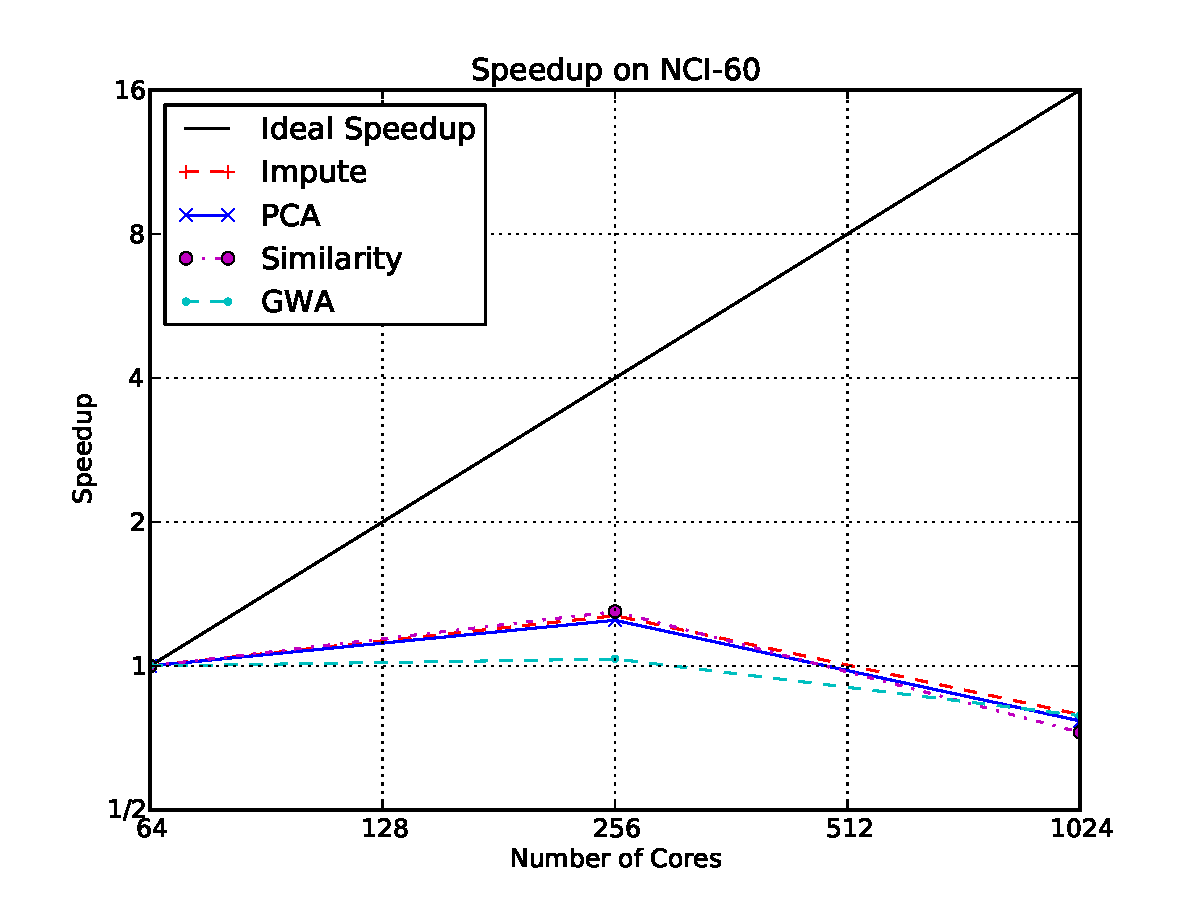
\includegraphics[width=0.5\linewidth]{graphs/speedup.pdf}
\end{center}
\caption{\textbf{A, left:} Runtime of the INDEL realignment and genotyping algorithms as the
number of cores is changed. Note that the times on the Y-axis are descending; as
the number of cores made available to \textsc{Avocado} is doubled, runtime
decreases. The dotted lines represent ideal scaling, where runtime halves when
the number of cores in the cluster is doubled. \textbf{B, right:} Job completion times
for the various stages of the \textsc{Avocado} pipeline.}
\label{fig:speedup}
\end{figure}

\textsc{Avocado} demonstrates linear strong scaling out to the full size of our
cluster. This is due to the even distribution of work across all of the nodes in
our cluster. This can be seen in Figure~\ref{fig:speedup}B, which shows that
task completion times are fairly uniform within each stage of the realignment
and genotyping process.

\section{Conclusion}
\label{sec:conclusion}

In this paper, we have introduced the indexed de Bruijn graph. This extension of the traditional
de Bruijn graph allows for $\Omega(n)$ local alignment of two or more sequences, with a hard
$\mathcal{O}(n)$ bound for canonical edits and an $\mathcal{O}(l^2)$ bound for non-canonical edits
(in genotyping, $l$ is the variant allele length, which is typically much smaller than $n$). After describing this structure, we have demonstrated how
indexed de Bruijn graphs can be used with a pooled model to locally reassemble haplotypes that contain
variants. By using an indexed de Bruijn graph, we are able to reduce the runtime complexity of the local
reassembly algorithms that are commonly used for variant discovery and calling.

\bibliographystyle{acm}
\bibliography{indexed-debruijn}

\end{document}
